%
\hsection{Defining and Assigning Variables}%
%
Like in mathematics, a variable in \python\ is basically a name with a value assigned to it.
You can define a variable and assign its value by writing \pythonil{name = value}.
Here, \pythonil{name} is the name of the variable and \pythonil{value} be the value that we want to assign to that name.%
%
\hsection{A Simple Example of Variable Assignment and Comments in the Code}%
\gitLoadAndExecPython{variables:assignment}{}{variables}{assignment.py}{}%
\listingPythonAndOutput{variables:assignment}{assignment.py}{%
A \python\ program showing some examples for variable assignments.}{}%
%
\begin{figure}[tb]%
\centering%
%
\subfloat[][%
\pythonil{int_var = 1}%
\label{fig:variable:assignment1}%
]{%
\strut\hspace{1.2cm}\strut%
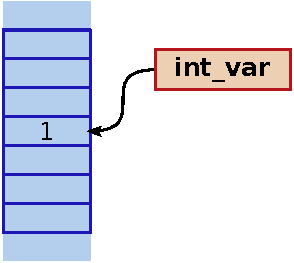
\includegraphics[width=0.23\linewidth]{\currentDir/assignment1}%
\strut\hspace{1.2cm}\strut}%
%
\floatSep%
%
\subfloat[][%
\pythonil{int_var = (3 * int_var) + 1}%
\label{fig:variable:assignment2}%
]{%
\strut\hspace{1.2cm}\strut%
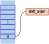
\includegraphics[width=0.23\linewidth]{\currentDir/assignment2}%
\strut\hspace{1.2cm}\strut}%
%
\\%
%
\subfloat[][%
\pythonil{float_var = 3.5}%
\label{fig:variable:assignment3}%
]{%
\strut\hspace{1.2cm}\strut%
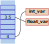
\includegraphics[width=0.23\linewidth]{\currentDir/assignment3}%
\strut\hspace{1.2cm}\strut}%
%
\floatSep%
%
\subfloat[][%
\pythonil{new_var = float_var * int_var}%
\label{fig:variable:assignment4}%
]{%
\strut\hspace{1.2cm}\strut%
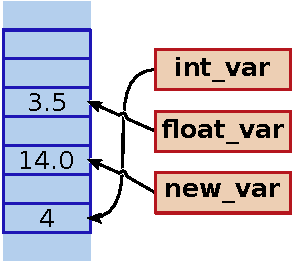
\includegraphics[width=0.23\linewidth]{\currentDir/assignment4}%
\strut\hspace{1.2cm}\strut%
}%
%
\caption{%
Illustrations of the variable assignments in \cref{lst:variables:assignment} in the same order in which they appear in the program: %
Variables are basically names that point to objects which are located somewhere in memory.}%
\label{fig:variable_assignment}%
\end{figure}%
%
\begin{figure}[tb]%
\centering%
%
\subfloat[][%
The file \textil{assignment.py} opened in \pycharm.%
\label{fig:assignmentPyCharm1}%
]{%
\tightbox{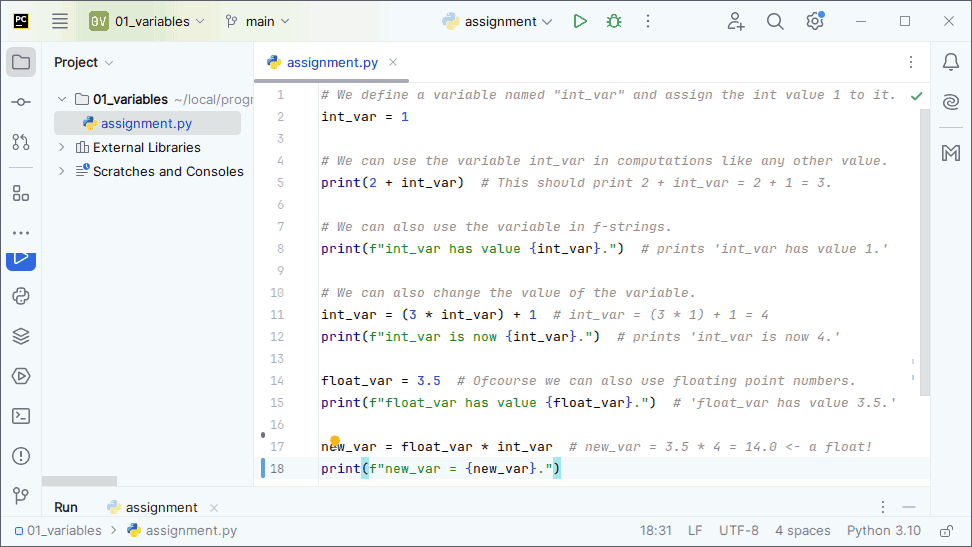
\includegraphics[width=0.49\linewidth]{\currentDir/assignmentPyCharm1}}%
}%
\hfill%
%
\subfloat[][%
Left-clicking on \menu{Run `assignment'} in the pop-up menu after right-clicking on \textil{assignment.py}, or directly pressing \keys{\ctrl+\shift+F10}, to run the program.%
\label{fig:assignmentPyCharm2}%
]{%
\tightbox{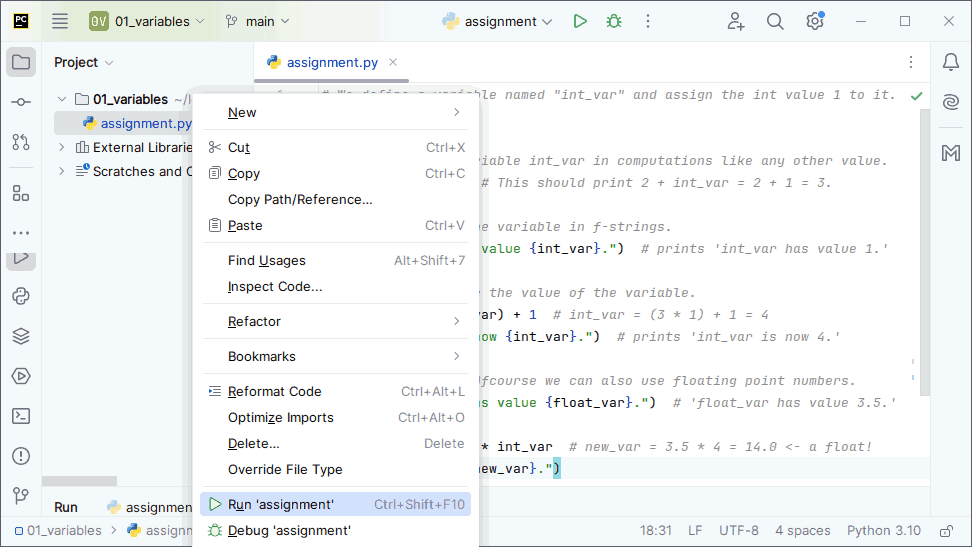
\includegraphics[width=0.49\linewidth]{\currentDir/assignmentPyCharm2}}%
}%
\\%
%
\subfloat[][%
The output of the program \textil{assignment.py} in \pycharm.%
\label{fig:assignmentPyCharm3}%
]{%
\tightbox{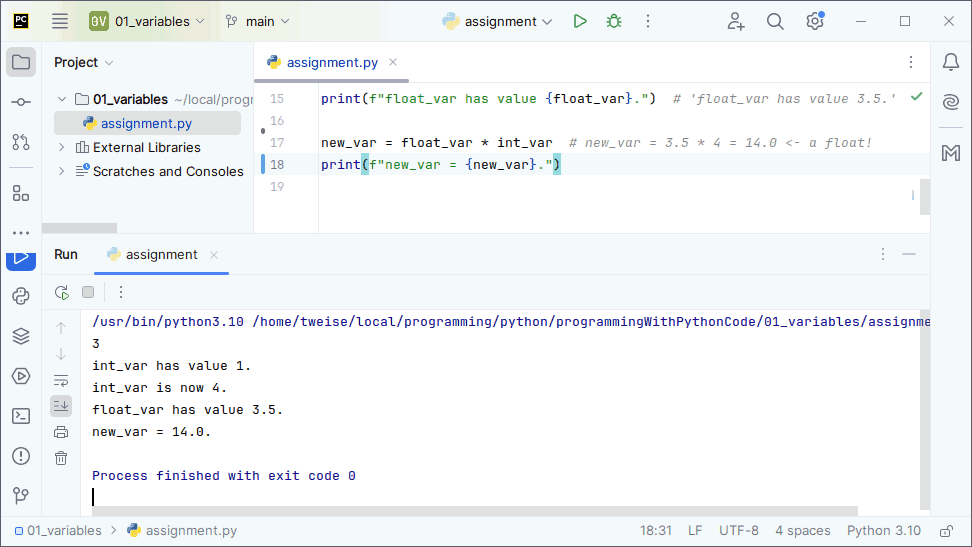
\includegraphics[width=0.7\linewidth]{\currentDir/assignmentPyCharm3}}%
}%
\\%
%
\subfloat[][%
The output of the program \textil{assignment.py} in the \ubuntu\ \pgls{terminal} (which you can open via~\ubuntuTerminal).%
\label{fig:assignmentTerminal}%
]{%
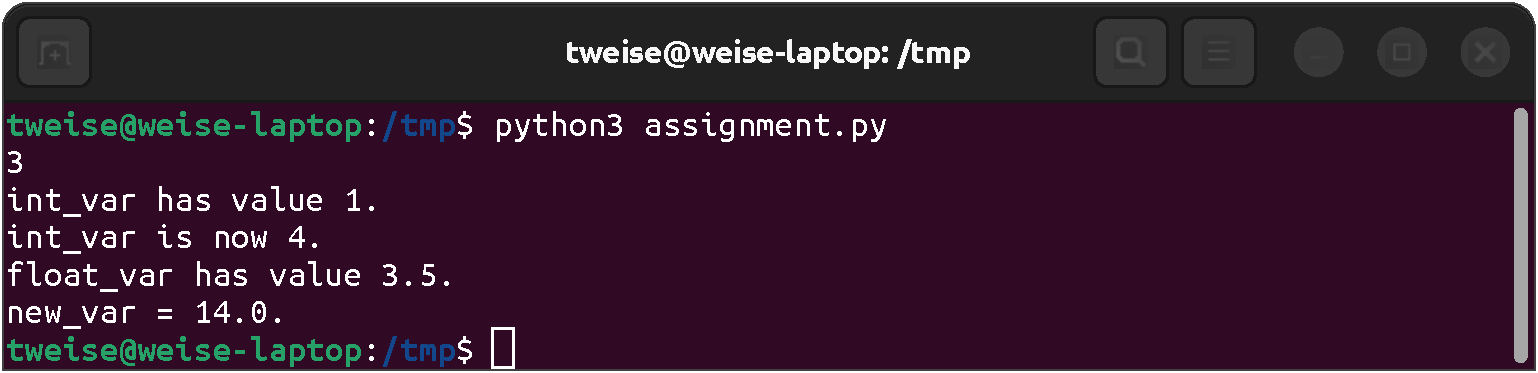
\includegraphics[width=0.7\linewidth]{\currentDir/assignmentTerminal}%
}%
%
\caption{Running the program \textil{assignment.py} from \cref{lst:variables:assignment} in \pycharm~(\cref{fig:assignmentPyCharm1,fig:assignmentPyCharm2,fig:assignmentPyCharm3}) or the \ubuntu\ \pgls{terminal}~(\cref{fig:assignmentTerminal}).}%
\label{fig:variables:assignment}%
\end{figure}%
%
With this, we can now store intermediate results.
This allows us, for the first time, two write programs that perform computations in multiple steps and that consist of multiple lines of code.%
%
\bestPractice{comments}{%
Comments help to explain what the code in programs does and are a very important part of the \emph{documentation} of code. %
Comments begin with a \pythonilIdx{\#} character, after which all text is ignored by the \python\ interpreter until the end of the current line. %
Comments can either occupy a complete line or we insert two spaces after the last code character in the line and then start the comment~\cite{PEP8}.%
}%
%
\cref{lst:variables:assignment} shows the source code of such a commented program.
This program does not do anything useful, but it illustrates how variables can be used.

It begins by assigning the \pythonilIdx{int} value~\pythonil{1} to a variable named~\pythonil{int_var}.
We could have chosen any other name as well, as long as it does not contain spaces, e.g., \pythonil{my_value}, \pythonil{cow}, \pythonil{race_car}.
But we chose \pythonil{int_var}.
The \pythonilIdx{=} assigns the value~\pythonil{1} to \pythonil{int_value}.
As \cref{fig:variable:assignment1} illustrates, the value~\pythonil{1} will now be stored somewhere in memory and \pythonil{int_var} is a name that points to this memory location.%
%
\begin{sloppypar}%
We can use \pythonil{int_var} just like any other value.
For example, we can compute \pythonil{2 + int_var} and pass the result to the \pythonilIdx{print} function.
This will then print \pythonil{3} to the \pgls{stdout} of our program.
We can also use \pythonil{int_var} in \pglspl{fstring}\pythonIdx{f-string}\pythonIdx{str!f} about which we learned back in \cref{sec:fstrings}.
\pythonil{f"int_var has value \{int_var\}."} will render to \pythonil{"int_var has value 1."}.%
\end{sloppypar}%
%
Variables are called \emph{variables} and not \emph{constants} because we can change their value.
Hence, we can update \pythonil{int_var} and give it a new value.
For example, we can do \pythonil{int_var = (3 * int_var ) + 1}.
As sketched in \cref{fig:variable:assignment2}, this will update \pythonil{int_var} to now hold the result of the computation \pythonil{(3 * int_var) + 1}.
In this computation, the current (old) value of \pythonil{int_var} is used.
It therefore corresponds to computing \pythonil{(3 * 1) + 1}, which equals~\pythonil{4}.
This value is stored somewhere in memory and \pythonil{int_var} points to it.
Doing \pythonil{print(f"int_var is now \{int_var\}.")} will print \textil{int_var is now 4.} to the \pgls{stdout}.
The value \pythonil{1} is now no longer referenced.
Eventually, the \python\ interpreter could free the corresponding memory to use it for something else.

Ofcourse, we can have multiple variables.
The command \pythonil{float_var = 3.5} creates a variable named \pythonil{float_var}.
It also allocates a piece of memory, writes the floating point value \pythonil{3.5} into it, and lets \pythonil{float_var} point to that piece of memory, as illustrated in \cref{fig:variable:assignment3}.
We can use this variable in an \pgls{fstring}\pythonIdx{f-string}\pythonIdx{str!f} as well:
\pythonil{print(f"float_var has value \{float_var\}.")} is interpolated to \pythonil{"float_var has value 3.5."}.%
%
\begin{sloppypar}%
In a final step, we create a third variables with the name \pythonil{new_var} by computing \pythonil{new_var = float_var * int_var}.
The result is \pythonil{3.5 * 4}, i.e., \pythonil{14.0}, \pythonilIdx{float} value.
\cref{fig:variable:assignment3} illustrates this variable assignment step.
Finally, \pythonil{print(f"new_var = \{new_var\}." )} then prints \textil{new_var = 14.0.}.%
\end{sloppypar}%
%
The \acrfull{stdout} of the complete program is given in \cref{exec:variables:assignment}.
For your convenience, we also showed the results when executing the program in \pycharm\ or the \ubuntu\ \pgls{terminal} in \cref{fig:variables:assignment}.
They are obviously identical.

Notice that we wrote the names of variables in a certain style, which is somewhat standard in \python\ programming.
For the sake of creating readable code that fits nicely together with code from other projects\dots%
%
\bestPractice{variableNames}{%
Variable names should be lowercase, with words separated by underscores~\cite{PEP8}.%
}
%
\FloatBarrier%
\endhsection%
%
\hsection{LIU Hui's Method and the Approximation of~$\numberPi$}%
\label{sec:approximatePiLiuHui}%
%
\begin{figure}%
\centering%
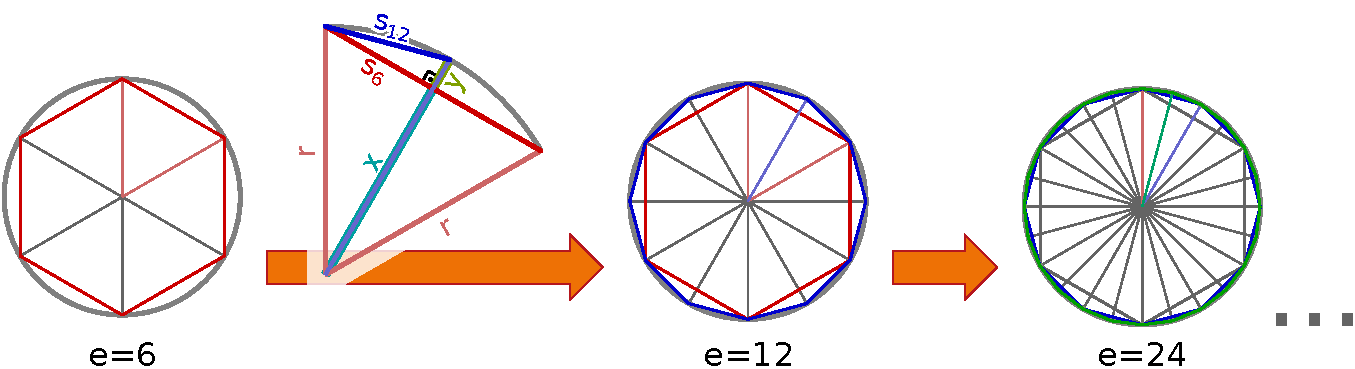
\includegraphics[width=0.99\linewidth]{\currentDir/liuHuiCircle}%
\caption{Approximating the ratio of the circumference and the diameter of a circle, i.e., $\numberPi$, by inscribing regular~$3*2^n$-gons.}%
\label{fig:liuHuiCircle}%
\end{figure}%
%
\definecolor{liuhui-r-color}{HTML}{CC6666}%
\def\liuhuir{\ensuremath{{\color{liuhui-r-color}r}}}%
\definecolor{liuhui-s6-color}{HTML}{CC0000}%
\def\liuhuiss{\ensuremath{{\color{liuhui-s6-color}s_6}}}%
\definecolor{liuhui-s12-color}{HTML}{0000CC}%
\def\liuhuist{\ensuremath{{\color{liuhui-s12-color}s_{12}}}}%
\definecolor{liuhui-y-color}{HTML}{80A000}%
\def\liuhuiy{\ensuremath{{\color{liuhui-y-color}y}}}%
\definecolor{liuhui-x-color}{HTML}{00A0A0}%
\def\liuhuix{\ensuremath{{\color{liuhui-x-color}x}}}%
\definecolor{liuhui-s24-color}{HTML}{00A000}%
\def\liuhuistf{\ensuremath{{\color{liuhui-s24-color}s_{24}}}}%
%
Let us now come to a more serious example.
I am not good at mathematics, but I really like mathematics anyway, so we will go with a mathematics example: approximating~\numberPi.
The number~\numberPi\ is the ratio of the circumference of a circle and its diameter.
A we already mentioned before in \cref{sec:float}, it is transcendental, a never-ending and never-repeating sequence of digits.
We can compute it to a certain precision, e.g., as the \pythonilIdx{float} constant \pythonilIdx{pi} with value \pythonil{3.141592653589793}.
But we can never really write it down.

Well, we I say \inQuotes{we can compute it}, then the question \inQuotes{How?} immediately arises.
One particularly ingenious answer was given by the Chinese mathematician LIU Hui~(刘徽) somewhere in the third century~AD~\cite{OR2003LH} in his commentary to the famous Chinese mathematics book \emph{Jiu Zhang Suanshu}~(九章算术)~\cite{OR2003LH,SCL1999TNCOTMACAC,S1998LHATFGAOCM,D2010AALHOCAS,C2002LFLHADWTDM}.
In \cref{fig:liuHuiCircle}, we show how~\numberPi, i.e., the ratio of the circumference and the diameter of a circle can be approximated by inscribing regular~$e$\nobreakdashes-gons into a circle.
The corners of the $e$\nobreakdashes-gons lie on the circle.

We start with a hexagon~($e=6$) where the radius~\liuhuir\ is equal to the radius of the circle.
All the $e$~edges~\liuhuiss\ of this hexagon then have length~\liuhuir\ as well.
It is easy to see that the circumference of the hexagon is~$U=e*\liuhuiss=6*\liuhuir$.
The diameter of the circle is~$D=2\liuhuir$.
Assuming that the circumference of the hexagon is an approximation of the circumference of the circle, we could approximate~\numberPi\ as $\numberPi\approx\frac{U}{D}$.
For $e=6$~edges, this gives us $\pi_6=\frac{6\liuhuir}{2\liuhuir}=3$.

Now this is a very coarse approximation of~\numberPi.
We can get closer to the actual ratio if we would use more edges, i.e., higher values of~$e$.
The ingenious idea of LIU Hui~(刘徽) is to use $e$\nobreakdashes-gons with~$e=3*2^n$.
For $n=1$, we get the hexagon with $e=6$.
For $n=2$, we double the edges and have a dodecagon with $e=12$~edges.
But how do we get the edge length~\liuhuist\ of this dodecagon?

We can get it from the edge length~\liuhuiss\ and radius~\liuhuir\ of the hexagon.
If we use the same six corners for the hexagon and dodecagon and connect the newly added six corners with the center of the circle, then these connections will separate each edge of the hexagon exactly in half and do so at a $90^\circ$~angle, as shown again in \cref{fig:liuHuiCircle}.
Here, the new side length~\liuhuist\ is the hypotenuse of a right-angled triangle with base~$\frac{\liuhuiss}{2}$ and height~\liuhuiy.
To get the height~\liuhuiy, we can use that~$\liuhuir=\liuhuix+\liuhuiy$ and the fact that there is a second right-angled triangle here, namely the one with base~\liuhuix, height~$\frac{\liuhuiss}{2}$, and hypotenuse~\liuhuir.
This gives us $\liuhuix^2+\left(\frac{\liuhuiss}{2}\right)^2=\liuhuir^2$.
Let's make things easier by choosing~$\liuhuir=1$.
We get $\liuhuix^2=1-\left(\frac{\liuhuiss}{2}\right)^2=1-\frac{\liuhuiss^2}{4}$ and, hence, $\liuhuiy=1-\sqrt{1-\frac{\liuhuiss^2}{4}}$.
With this we can move on to $\liuhuist^2=\liuhuiy^2+\left(\frac{\liuhuiss}{2}\right)^2$, which we can resolve to $\liuhuist^2=\left(1-\sqrt{1-\frac{\liuhuiss^2}{4}}\right)^2+\frac{\liuhuiss^2}{4}$.
Using $(a-b)^2=a^2-2ab+b^2$ and applying it to the first term, we get $\liuhuist^2=1-2\sqrt{1-\frac{\liuhuiss^2}{4}}+\left(1-\frac{\liuhuiss^2}{4}\right)+\frac{\liuhuiss^2}{4}$.
This then gives us $\liuhuist^2=2-2\sqrt{1-\frac{\liuhuiss^2}{4}}-\frac{\liuhuiss^2}{4}+\frac{\liuhuiss^2}{4}$, which we can further refine to $\liuhuist^2=2-2\sqrt{1-\frac{\liuhuiss^2}{4}}$.
We can pull th~$2$ from outside the root into the root by multiplying everything inside by $2^2=4$ and get $\liuhuist^2=2-\sqrt{4-\liuhuiss^2}$.
Thus, we have the really elegant $\liuhuist=\sqrt{2-\sqrt{4-\liuhuiss^2}}$.

As new approximation of~$\pi_{12}$, we now have $\frac{12*\liuhuist}{2\liuhuir}=6*\liuhuist=6\sqrt{2-\sqrt{4-\liuhuiss^2}}=6\sqrt{2-\sqrt{4-1}}=6\sqrt{2-\sqrt{3}}\approx 3.105828539$.
This is already quite nice.
We can actually repeat this step to get to~\liuhuistf.
And we could continue this process by again doubling the number the edges.
Repeating the above calculations and observing \cref{fig:liuHuiCircle}, we get the equation:%
%
\begin{align}%
s_{2e} &= \sqrt{2-\sqrt{4-s_e^2}}\label{eq:liuhui:sidelength}\\%
\pi_{2e} &= \frac{e}{2} s_{2e}\label{eq:liuhui:approx}%
\end{align}%
%
\gitLoadAndExecPython{variables:pi_liu_hui}{}{variables}{pi_liu_hui.py}{}%
\listingPythonAndOutput{variables:pi_liu_hui}{file}{%
A \python\ program showing several steps of the approximation of~\numberPi\ using the method of LIU Hui~(刘徽).}{}%
%
\begin{figure}[tb]%
\centering%
%
\subfloat[][%
The file \textil{pi_liu_hui.py} opened in \pycharm.%
\label{fig:liuHuiPiPyCharm1}%
]{%
\tightbox{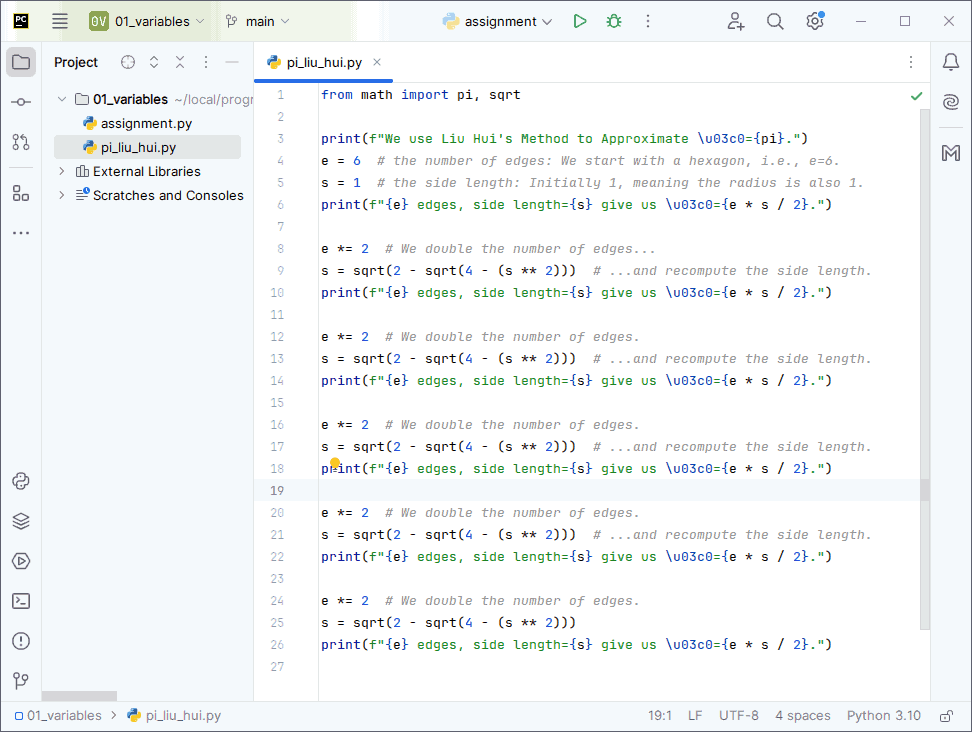
\includegraphics[width=0.49\linewidth]{\currentDir/liuHuiPiPyCharm1}}%
}%
\hfill%
%
\subfloat[][%
Left-clicking on \menu{Run `pi\_liu\_hui'} in the pop-up menu after right-clicking on \textil{pi_liu_hui.py}, or directly pressing \keys{\ctrl+\shift+F10}, to run the program.%
\label{fig:liuHuiPiPyCharm2}%
]{%
\tightbox{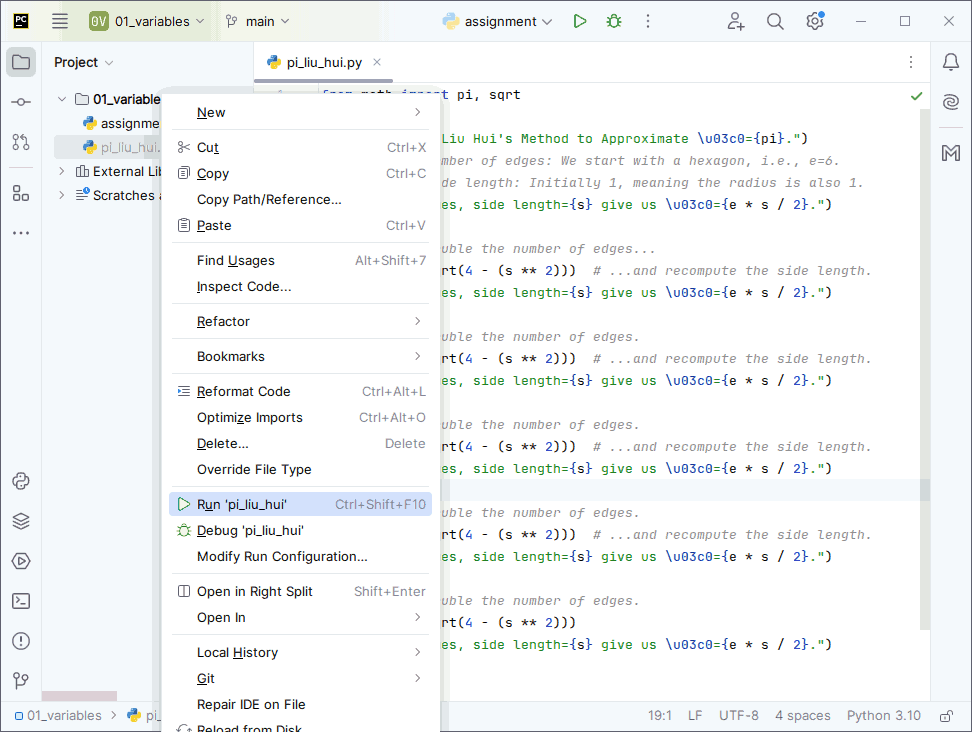
\includegraphics[width=0.49\linewidth]{\currentDir/liuHuiPiPyCharm2}}%
}%
\\%
%
\subfloat[][%
The output of the program \textil{pi_liu_hui.py} in \pycharm.%
\label{fig:liuHuiPiPyCharm3}%
]{%
\tightbox{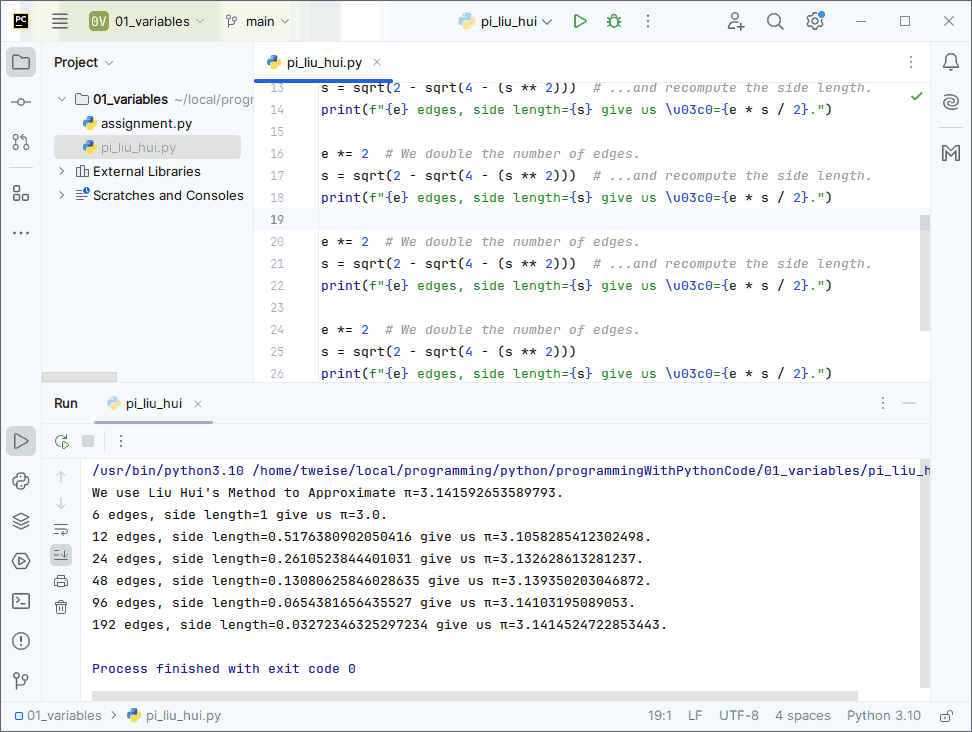
\includegraphics[width=0.7\linewidth]{\currentDir/liuHuiPiPyCharm3}}%
}%
\\%
%
\subfloat[][%
The output of the program \textil{pi_liu_hui.py} in the \ubuntu\ \pgls{terminal} (which you can open via~\ubuntuTerminal).%
\label{fig:liuHuiPiTerminal}%
]{%
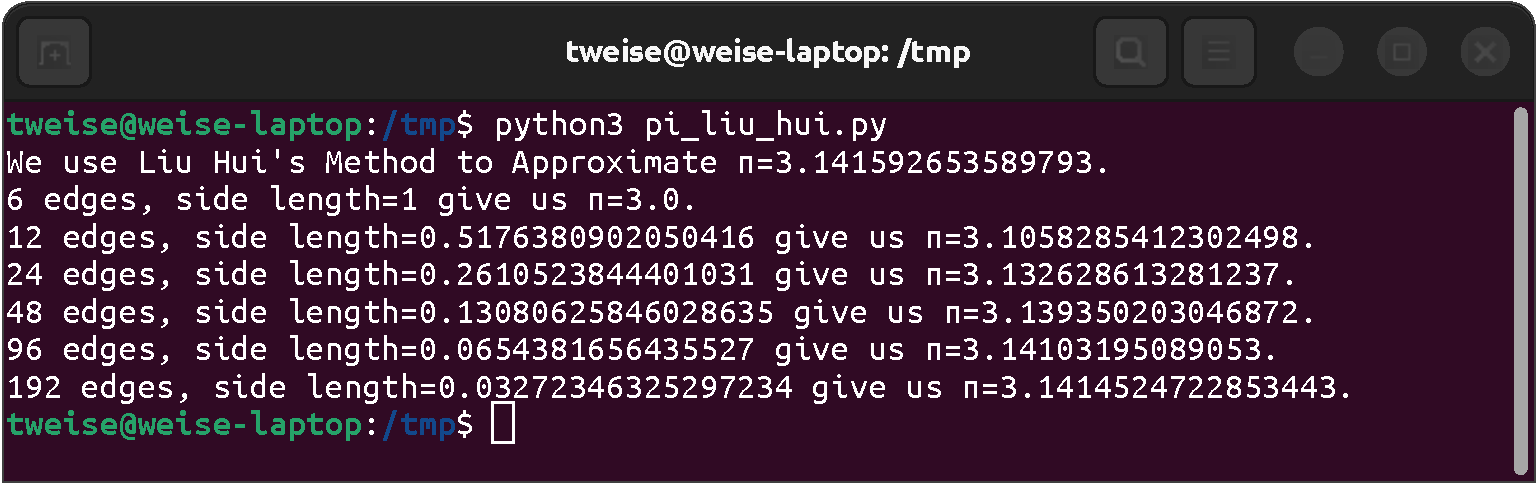
\includegraphics[width=0.7\linewidth]{\currentDir/liuHuiPiTerminal}%
}%
%
\caption{Running the program \textil{pi_liu_hui.py} from \cref{lst:variables:assignment} in \pycharm~(\cref{fig:assignmentPyCharm1,fig:assignmentPyCharm2,fig:assignmentPyCharm3}) or the \ubuntu\ \pgls{terminal}~(\cref{fig:assignmentTerminal}).}%
\label{fig:variables:liuHuiPi}%
\end{figure}%
%
Now that we have learned some programming, we do no longer need to type the numbers and computation steps into a calculator.
Instead, we can simply write them into a program, as illustrated in \cref{lst:variables:pi_liu_hui}.
We begin by setting the number of edges \pythonil{e = 6} and the side length to \pythonil{s = 1}, still choosing~$\liuhuir=1$.
In each iteration of the approximation, we simply set \pythonil{e *= 2}\pythonIdx{*=}, which is equivalent to \pythonil{e = e * 2}, to double the number of edges.
We compute \pythonil{s = sqrt(2 - sqrt(4 - (s ** 2)))}\pythonIdx{sqrt} having imported\pythonIdx{import} the \pythonilIdx{sqrt} function from the \pythonilIdx{math} module.
We print the approximated value of~\numberPi\ as \pythonil{e * s / 2}.
Notice how elegantly we use the unicode characters~$\pi$ and~$\approx$ via the escapes~\pythonil{\\u03c0} and \pythonil{\\u2248}\pythonIdx{\textbackslash{u}}, respectively, from back in~\cref{sec:unicodeChars} (and how nicely it indeed prints the greek character~$\pi$ in the \pgls{stdout} in \cref{exec:variables:pi_liu_hui}).
Either way, since \cref{eq:liuhui:sidelength,eq:liuhui:approx} are always the same, we can simply copy-paste the lines of code for updating~\pythonil{s}, \pythonil{e}, and printing the approximated value of~\numberPi\ several times.

\Cref{exec:variables:pi_liu_hui} shows the \acrfull{stdout} produced by this program.
Indeed, each new approximation comes closer to~\numberPi.
For 192~edges, we get the approximation~\pythonil{3.1414524722853443}.
Given that the constant~\pythonilIdx{pi} from the \pythonilIdx{math} module is \pythonil{3.141592653589793}, we find that the first four digits are correct and that the number is only off by only 0.0045\%!
For your convenience, we also showed the results when executing the program in \pycharm\ or the \ubuntu\ \pgls{terminal} in \cref{fig:variables:liuHuiPi}.
They are obviously identical.
Therefore, in the future, we will only very sporadically add such screenshots.
Instead, we will usually only print code and output pairs like~\cref{lst:variables:pi_liu_hui,exec:variables:pi_liu_hui}.%
%
\endhsection%
%
\FloatBarrier%
\endhsection%
%
